\section{}
A crane 100 m tall is loading a container full of feathers and delicate glass figurines weighing 5 metric tons onto a cargo ship. While the container is in the air, there is an emergency shutdown of the crane and the case is left hanging for a short time. During this time, winds cause the arm of the crane to vibrate vertically at a frequency of 4 Hz with an amplitude of 5 cm. The supporting cable has an effective stiffness of $k = \frac{100}{L}$ MN/m, where $L$ is the length of exposed cable in metres (neglect changes in $L$ due to vibration).

\begin{figure}[h]
\centering
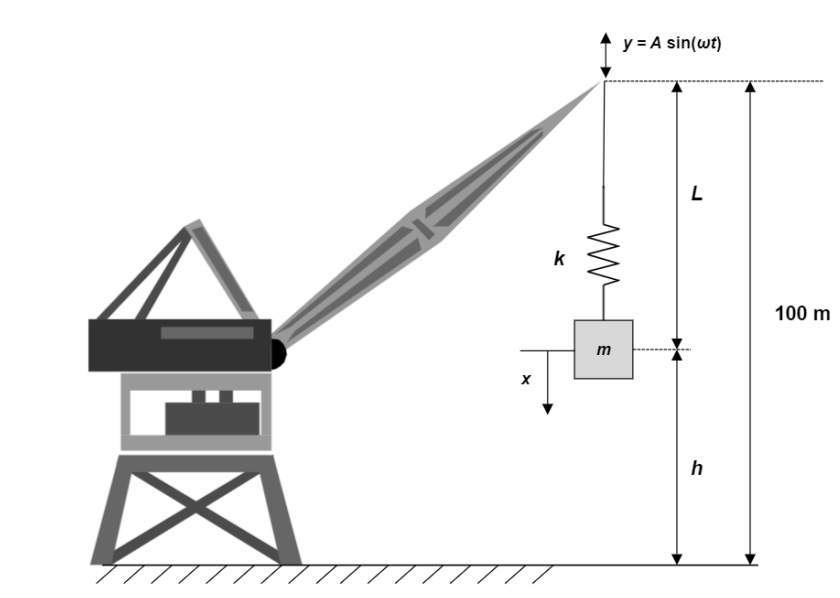
\includegraphics[width=0.5\textwidth]{Questions/Figures/q2 problem diagram.png}
\end{figure}
\FloatBarrier
\begin{enumerate}[label=(\alph*)]
    \item (2 pts) Determine the cable length $L$ at which the transmissibility would be exactly 1.
    \item (5 pts) Assuming steady state vibration, determine all possible heights $h$ at which the crate would hit the ground.
    \item (3 pts) After the emergency is dealt with, operations resume as the wind continues to excite the crane arm. The crane needs to lift shipments 80 m high to place it onto the cargo ships. What is the smallest mass of cargo that can be lifted in these conditions without shaking with an amplitude greater than 4 cm? Assume $\omega > p$.
\end{enumerate}
\FloatBarrier
\subsection*{Solution}
\subsection{}
First, we must choose the proper model for the system. A simple undamped spring-mass with base excitation model is appropriate. Assume the weight of the cable is negligible. 

The transmissibility is then
\begin{align*}
    \text{TR} &= \frac{\left(\frac{\omega}{p}\right)^2}{1 - \left(\frac{\omega}{p}\right)^2} \\
\end{align*}
converting $f = 4$ Hz to $\omega = 2\pi f = 8\pi$ rad/sec, we can solve for $p$ when $\text{TR} = 1$
\begin{align*}
    1 &= \frac{\left(\frac{8\pi}{p}\right)^2}{1 - \left(\frac{8\pi}{p}\right)^2} \\
    1 - \left(\frac{8\pi}{p}\right)^2 &= \left(\frac{8\pi}{p}\right)^2 \\
    1 &= 2\left(\frac{8\pi}{p}\right)^2 \\
    \implies p &= 8\sqrt{2} \pi
\end{align*}
Since $p$ is defined as 
\begin{align*}
    p &= \sqrt{\frac{k}{m}}\\
    \implies k &= p^2m \\
    &= (8\sqrt{2}\pi)^2 (5 \times 10^3) \\
    &= 0.64\pi^2 \times 10^6 \text{ N/m} \\
    &= 0.64\pi^2 \text{ MN/m}
\end{align*}
and since $k = \frac{100}{L}$, we can solve for $L$,
\begin{align*}
    \Aboxed{L &= \frac{100}{k} = \frac{100}{0.64\pi^2} = 15.8 \text{ m}}
\end{align*}

\subsection{}
% redoing with better method
The DMF is
\begin{align*}
    \frac{\mathbb{X}}{\mathbb{X}_0} &= \frac{1}{\bigg| 1 - \left(\frac{\omega}{p}\right)^2 \bigg|}
\end{align*}
Since we want the amplitude to be equal to or greater than the height of the crate, we're interested in the region between resonance and the value where the amplitude is equal to the height of the crate. 
\begin{figure}[h]
    \centering
    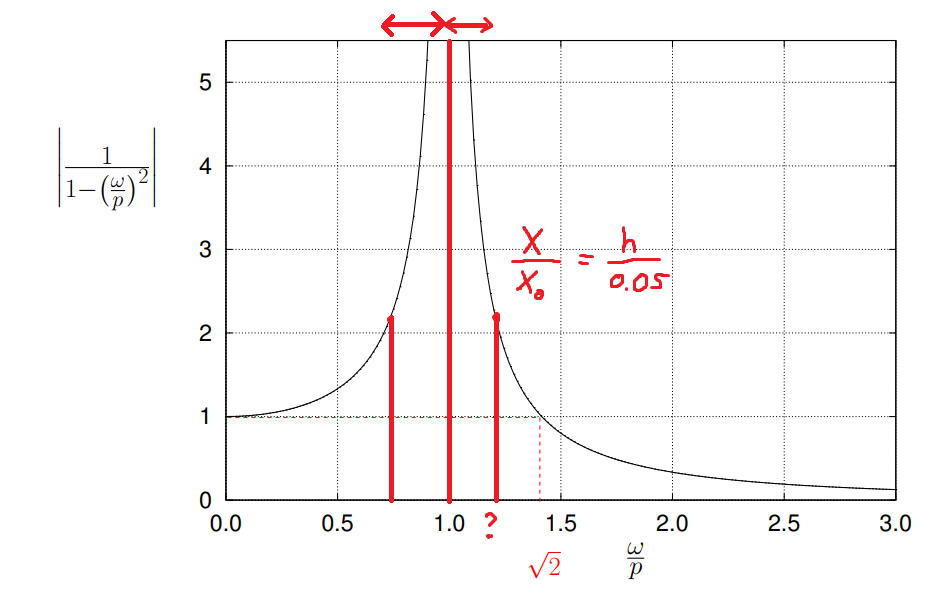
\includegraphics[width=0.5\textwidth]{Questions/Figures/q2 dmf.png}
    \caption{Operating range for b)}
\end{figure}
First, let us find the point past resonance where the DMF is 
\begin{align*}
    \text{DMF} := \frac{\mathbb{X}}{\mathbb{X}_0} &= \frac{h}{0.05} \\
    &= \frac{1}{\bigg| 1 - \left(\frac{\omega}{p}\right)^2 \bigg|} \\
    &= \frac{1}{\bigg| 1 - \frac{m\omega^2}{k} \bigg|} \\
    &= \frac{1}{\bigg| 1 - \frac{mL\omega^2}{100 \times 10^6} \bigg|} \\
    &= \frac{1}{\bigg| 1 - \frac{m(100 - h)\omega^2}{10^8} \bigg|} \\
    &= \frac{1}{\bigg| 1 - \frac{5 \times 10^3(100 - h)(8\pi)^2}{10^8} \bigg|} \\
\end{align*}
\begin{verbatim}
syms h
eqn = 1/abs(1 - 5*10^3*(100-h)*(8*pi)^2/10^8) == h/0.05;
h = solve(eqn, h);
h = double(h)

>> h =
        0.0232
        68.3140
        68.3603
\end{verbatim}
The natural frequency at each of these points is
\begin{align*}
    p &= \sqrt{\frac{100}{(100-h)m} \times 10^6} \\
    p_1 &= \sqrt{\frac{100}{(100 - 0.0232) \times 5 \times 10^3} \times 10^6} = 14.144 \\
    p_2 &= \sqrt{\frac{100}{(100 - 68.314) \times 5 \times 10^3} \times 10^6} = 25.124 \\
    p_3 &= \sqrt{\frac{100}{(100 - 68.3603) \times 5 \times 10^3} \times 10^6} = 25.142 
\end{align*}
Since the driving frequency is 8$\pi = 25.133$, and $\omega > p$, the only solution is $68.3403$ m.

Now let's solve for resonance. This happens when the DMF is infinite, or when the denominator is zero. Then,
\begin{align*}
    1 - \frac{m(100 - h)\omega^2}{10^8} &= 0 
\end{align*}
\begin{verbatim}
syms h
eqn = 1 - 5*10^3*(100-h)*(8*pi)^2/10^8 == 0;
h = solve(eqn, h);
h = double(h)

h =
    68.3371
\end{verbatim}
So the possible heights are $\boxed{h = (68.337, 68.360] \text{ m}}$.

\subsection{}
Let $h = 80$, and the operating range is $\omega > p$. Then, the DMF is
\begin{align*}
    \text{DMF} &= \frac{1}{\left(\frac{\omega}{p}\right)^2 - 1}
\end{align*}
Since the shaking specification is 4 cm, then
\begin{align*}
    \frac{4}{5} &= \frac{1}{\left(\frac{\omega}{p}\right)^2 - 1} \\
    \frac{4}{5} &= \frac{1}{\left(\frac{8\pi}{p}\right)^2 - 1} \\
\end{align*}
Solving for $p$, 
\begin{verbatim}
syms p
eqn = 4/5 == 1/((8*pi/p)^2 - 1);
p = solve(eqn, p);
p = double(p)

>> p = -15.7003
        15.7003
\end{verbatim}
The only physical solution is $p = 15.7$ rad/sec.
By the definition of $p$,
\begin{align*}
    p &= \sqrt{\frac{k}{m}} \\
    &= \sqrt{\frac{100/L \times 10^6}{m}} 
\end{align*}
Solving for $m$,
\begin{align*}
    m &= \frac{100/L \times 10^6}{p^2} \\
    &= \frac{100/20 \times 10^6}{(15.7)^2} \\
    &= \boxed{20.28 \times 10^3 \text{ kg}}
\end{align*}
